% Chapter Template

\chapter{Demonstrating the Tool} % Main chapter title

\label{Chapter6} % Change X to a consecutive number; for referencing this
% chapter elsewhere, use \ref{ChapterX}

\lhead{Chapter 6. \emph{Demonstrating the Tool}} % Change X to a consecutive
% number; this is for the header on each page - perhaps a shortened title

This section considers a specific example of an exogenous model to model
transformation and is similar to the case study that was covered in
section~\ref{tools}. The source DSML is defined according to two abstraction
layers while the target DSML is defined according to one abstraction layer. This
section will consider the most significant parts of the workflow of a model
transformation for the DPF Transformation Editor that was described in
figure~\ref{fig:work_flow_solution} in section~\ref{integrate_henshin}.

\begin{figure}[H]
	\centering
	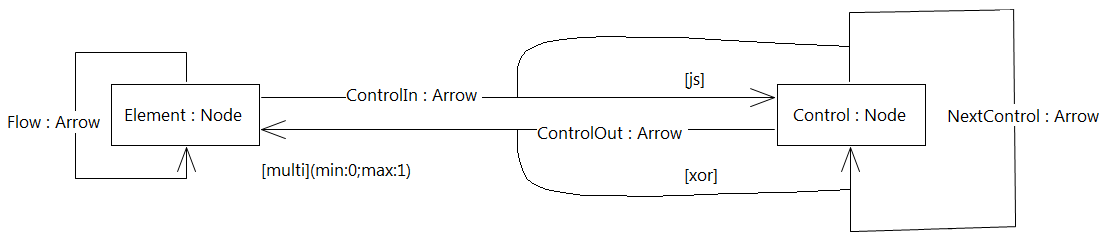
\includegraphics[scale=0.5]{./Figures/DPFactivityMetamodel_1.png}
	\caption[Source modeling formalism one abstraction layer higher]
	{Modeling formalism at $\spec{S}$\textsubscript{3} abstraction layer.}
	\label{fig:source_DSL_1}
\end{figure}

Figure~\ref{fig:source_DSL_1} represents a modeling formalism for an activity
diagram that is defined in abstraction layer $\spec{S}$\textsubscript{3}. The
figure includes the two nodes Element and Control and the four arrows ControlIn,
ControlOut, NextControl and Flow. The semantics of the model is specified by
defining a couple of predicates for the arrows. The \textit{[js]} specifies that
a Control should have at least one incomming arrow from an Element or Control.
The \textit{[xor]} specifies that a Control can have either have an outgoing
arrow to an Element or another Control both not to both. The multiplicity
predicate specifies that a Control can only be connected with maximum one other
Element. The specification $\spec{S}$\textsubscript{3} together with the
constraints that are defined specifies a modeling formalism for a DPF
specification one abstraction layer lower.

\begin{figure}[H]
	\centering
	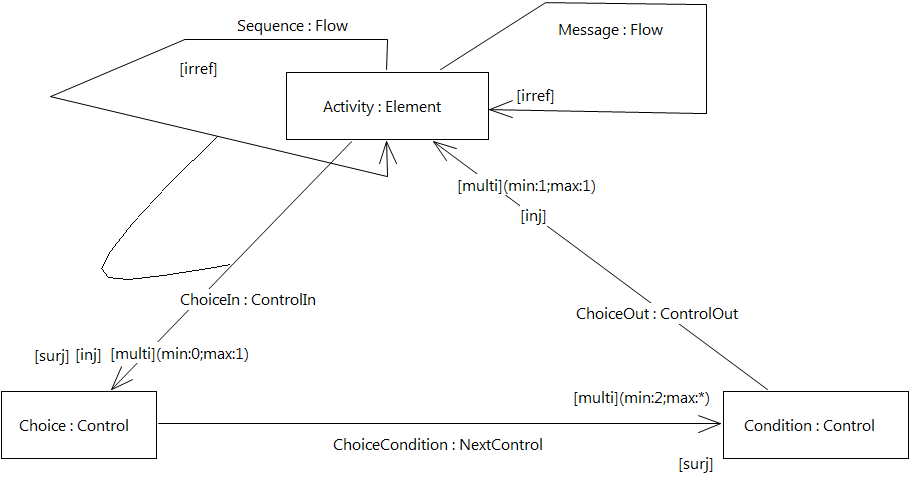
\includegraphics[scale=0.5]{./Figures/DPFactivityMetamodel_2.png}
	\caption[Source modeling formalism]
	{Source modeling formalism at $\spec{S}$\textsubscript{2} abstraction layer.}
	\label{fig:source_DSL_2}
\end{figure}

Figure~\ref{fig:source_DSL_2} represents a set of predicates for a specification
$\spec{S}$\textsubscript{2} that conforms to the modeling formalism specified in
figure~\ref{fig:source_DSL_1}. This modeling formalism consists of one Element
and two Control domain classes. The semantic of the modeling formalism is
specified by a set of predicates and arrows between the three domain classes.
The predicates for an Activity specifies that an Activity never can relate to
itself but can relate to other Activity elements. A Choice and a Condition
element is required to be connected with exactly one Activity element while a
each Choice element requires a connection with at least two Condition elements.
This modeling formalism represents the meta-model that describes the source DPF
specification $\spec{S}$\textsubscript{1} for this exogenous model
transformation.

\begin{figure}[H]
	\centering
	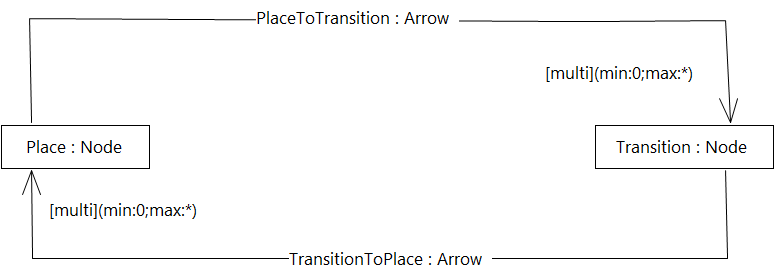
\includegraphics[scale=0.5]{./Figures/DPFpetrinet.png}
	\caption[Target modeling formalism]
	{Target modeling formalism at $\spec{S}$\textsubscript{2} abstraction layer.}
	\label{fig:target_DSL_1}
\end{figure}

Figure~\ref{fig:target_DSL_1} represents the modeling formalism for a
Petri net model and is the meta-model for the target DPF specification. The
modeling formalism specifies that two domain classes Place and Transition can
be connected to each other with a TransitionToPlace and a PlaceToTransition
arrow. Note that both the modeling formalism presented in this figure and
figure~\ref{fig:source_DSL_1} conforms to the default DPF specification that is
a Node connected with itself.

So far we have covered step 1 by defining a source and target modeling formalism
of a model transformation in the DPF Transformation Editor. The next step is to
define a new isntance of a model transformation that initializes an empty
correspondence graph and the joined modeling formalism. Step 3 focus on creating
a set of transformation rules and specify the correspondence objects between
source and target modeling formalism. Henshin requires this relation to be able
to perform an exogenous model transformation.
Figure~\ref{fig:correspondence_arrow} illustrates that all arrows in the source
modeling formalisms should be translated according to a Place in the target
modeling formalism.

\begin{figure}[H]
	\centering
	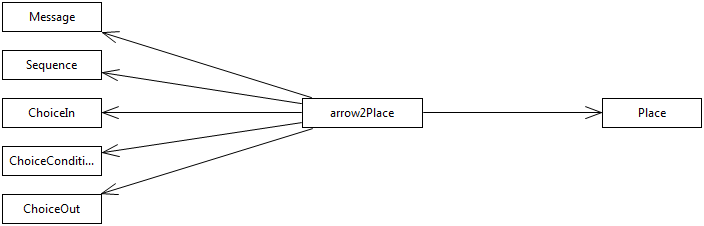
\includegraphics[scale=0.6]{./Figures/correspondenceObjects.png}
	\caption[Simplified joined specification]
	{Correspondence of modeling objects in source and target modeling formalisms.}
	\label{fig:correspondence_arrow}
\end{figure}

Note that this will jeopardize the semantics of the source and target modeling
formalism by stating that an arrow should be translated to a node. However, to
simplify an exogenous model transformation we specify that arrows from a source
modeling formalism should correspond to a Place. The idea behind specifying the
correspondence between objects is that the user is responsible for how a target
specification is produced. The next part of step 3 is to define a set of
transformation rules. Figure~\ref{fig:rule_collection} defines that eight
transformation rules is needed to translate an instance specification of the
source modeling formalism. 

\begin{figure}[H]
	\centering
	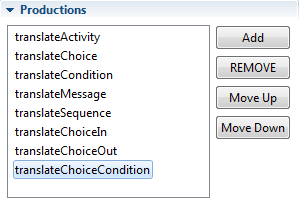
\includegraphics[scale=0.7]{./Figures/transformationrules_solution.png}
	\caption[Collection of rules in the DPF Transformation Editor.]
	{The set of transformation rules for this specific model transformation.}
	\label{fig:rule_collection}
\end{figure}

Figure~\ref{fig:translateCond_translateChoic} illustrates the two rules
translateCondition and translateChoice. For the first rule we specify that a
Condition modeling element from the source modeling formalism should be part of
the searching pattern while a Trace and Transition modeling element are created
for each located matching pattern.

\begin{figure}[H]
	\centering
	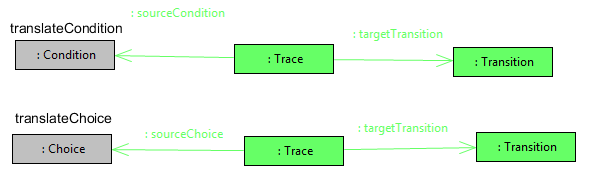
\includegraphics[scale=0.7]{./Figures/translateChoice_Condition.png}
	\caption[Transformation rules created in the integrated view.]
	{The transformation rules translateCondition and translateChoice.}
	\label{fig:translateCond_translateChoic}
\end{figure}

Trace specifies the correspondence between source and target modeling elements
and represents a traceable link with a source and target modeling element. Note
that the color gray specifies that modeling elements belongs to the
intersection graph while the color green specifies that modeling elements are
part of the RHS graph. Figure~\ref{fig:integratedView_rule} illustrates the
integrated view for editing transformation rules in the DPF Transformation
Editor. The Palette on the right side includes the modeling elements that is
provided from the joined modeling formalism that was generated accordingly to
step 2. 

\begin{figure}[H]
	\centering
	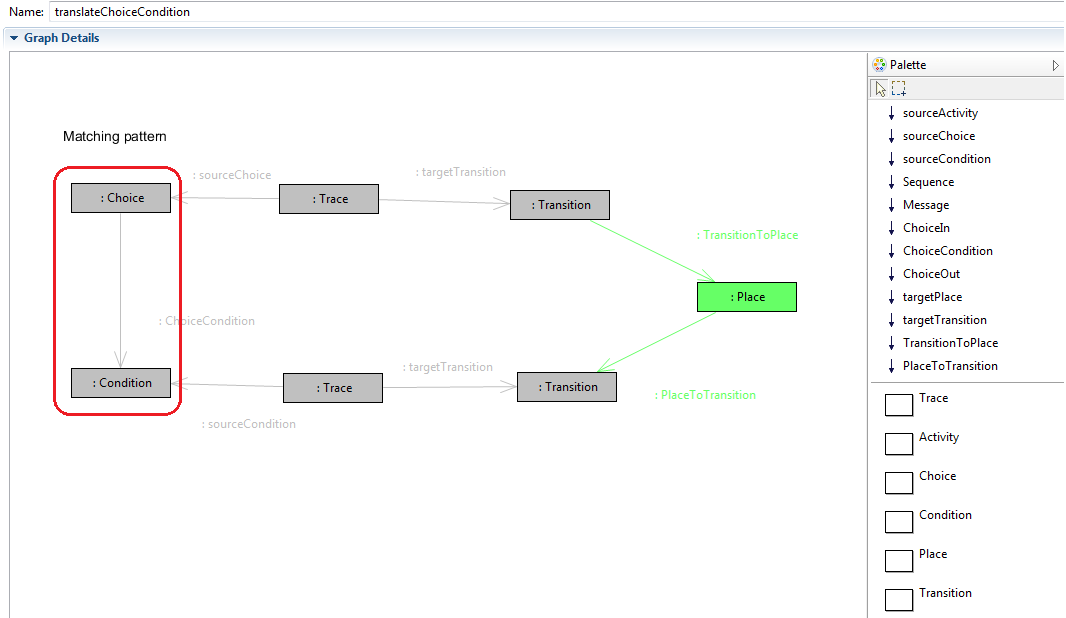
\includegraphics[scale=0.5]{./Figures/translateChoiceCondition.png}
	\caption[Integrated view for the DPF Transformation Editor]
	{The integrated view for a specific transformation rule.}
	\label{fig:integratedView_rule}
\end{figure}

Before we describe the semantics of this specific transformation rules we should
illustrate what matching pattern the rule searches for.

\begin{figure}[H]
	\centering
	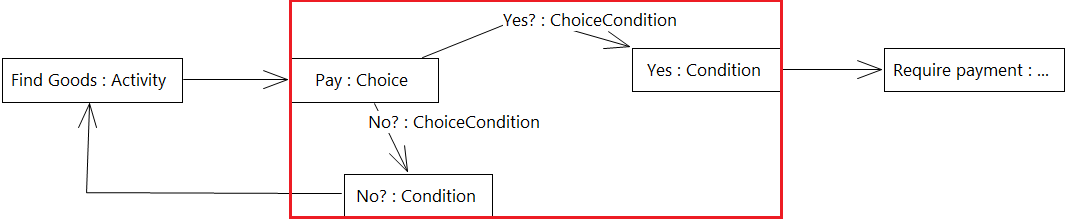
\includegraphics[scale=0.5]{./Figures/isntanceExmaple.png}
	\caption[Small fragment of the source model]
	{A small fragment of the source model for this specific model transformation.}
	\label{fig:fragment_instance}
\end{figure}


Figure~\ref{fig:fragment_instance} represents a small fraction of the source
model that will be translated. In this rule we want to locate a matching pattern
that has a Choice connected with a Condition by a ChoiceCondition. Note that
this specific rule will locate two matching pattern when applied. The first
matching pattern is when the Choice is Yes while the second matching pattern is
when the Choice is No. Back to the specific transformation rule,
``translateChoiceCondition'' in figure~\ref{fig:integratedView_rule}. We have a
matching pattern that is part of the intersection graph. The matching pattern
locates matches that has a Choice connected with a Condition by a
ChoiceCondition. This rule will locate two different matches as shown in 
figure~\ref{fig:fragment_instance}. The rule also specifies that a Place
and two arrows are produced for every located matching pattern. One thing that
is special for this rule is that two trace and transition modeling elements are
part of the intersection graph. This is because these modeling elements already
have been translated in the two transformation rules that were defined in
figure~\ref{fig:translateCond_translateChoic}. The two traces specifies that the
two Transition elements corresponds to a Choice and a Condition element that is
already translated for these matches. The newly created Place element are
connected with the two already translated Transform elements with a
TransitionToPlace and a PlaceToTransform arrow. The two final steps of the
workflow of consist of generating a set of Henshin transformation rules from the
eight rules in the DPF Transformation Editor and applying the Henshin rules to a
source model. 

\begin{figure}[H]
	\centering
	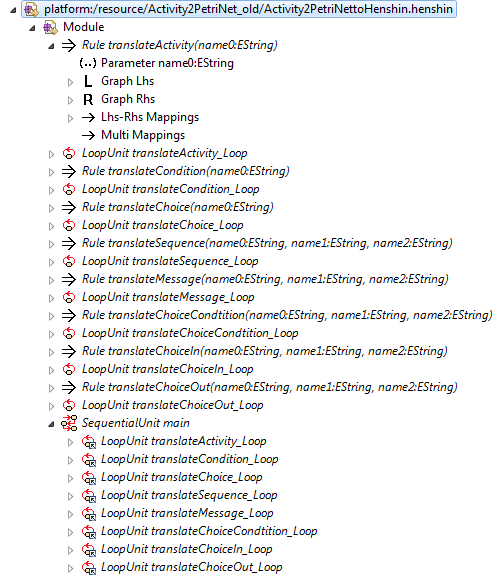
\includegraphics[scale=0.7]{./Figures/henshin_rules.png}
	\caption[A collection of a set of produced Henshin rules]
	{The eight transformation rules generated in Henshin.}
	\label{fig:henshin_rules}
\end{figure}

Figure~\ref{fig:henshin_rules} represents a generated Henshin module with eight
transformation rules. Each rule has a LHS, a RHS graph and a collection of
mappings that forms the intersection graph. The parameter name0 for the
``translateActivity'' is used to pass along a variable from one matching
modeling element to a produced target modeling element. Note that there are a
collection of 17 items for this Module. The SequentailUnit, main represents the
scheduling mechanism that specifies that 8 LoopUnits is applied in sequential
order. Each LoopUnit has a corresponding transformation rule as subunit. The
rules are applied until there are exist no more matching patterns. The main
sequential unit can be applied to a source model and translate is according to
the rules for a Henshin module. After the transformation we can extract the
translated target modeling elements and explicitly assign these modeling
elements to the target modeling formalism. 

\begin{figure}[H]
	\centering
	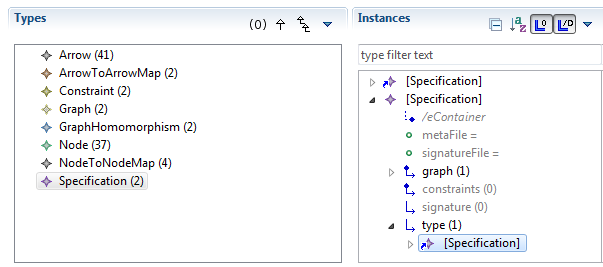
\includegraphics[scale=0.7]{./Figures/translated_model.png}
	\caption[The translated model for the case study.]
	{The result of this specific exogenous model transformation.}
	\label{fig:translated_model}
\end{figure}

Figure~\ref{fig:translated_model} represents the translated DPF specification
that conforms to a target modeling formalism. The Node and Arrows represents the
translated modeling elements that is named according to matched modeling
elements. 
